%
% Erstellt von Daniel Falkner
% bmw@740i.de
% 
\documentclass[xcolor=dvipsnames]{beamer}
\usepackage[T1]{fontenc}
\usepackage[utf8]{inputenc}
\usepackage[ngerman]{isodate}
\usepackage[justification=centering,figurename=Abb.]{caption}
\usepackage{listings}
\usepackage{color}


\definecolor{mygreen}{rgb}{0,0.6,0}
\definecolor{mygray}{rgb}{0.5,0.5,0.5}
\definecolor{mymauve}{rgb}{0.58,0,0.82}

\lstdefinelanguage{JavaScript}{
  keywords={break, case, catch, continue, debugger, default, delete, do, else, finally, for, function, if, in, instanceof, new, return, switch, this, throw, try, typeof, var, void, while, with},
  morecomment=[l]{//},
  morecomment=[s]{/*}{*/},
  morestring=[b]',
  morestring=[b]",
  sensitive=true
}

\lstdefinelanguage{CSS}
{morekeywords={color,background,margin, font, width, float, height, padding, box, opacity, border, right, top, shadow, radius, bottom},
sensitive=false,
morecomment=[l]{//},
morecomment=[s]{/*}{*/},
morestring=[b]",
} 

\lstset{ %
  backgroundcolor=\color{white},   % choose the background color; you must add \usepackage{color} or \usepackage{xcolor}
  basicstyle=\footnotesize,        % the size of the fonts that are used for the code
  breakatwhitespace=false,         % sets if automatic breaks should only happen at whitespace
  breaklines=true,                 % sets automatic line breaking
  captionpos=b,                    % sets the caption-position to bottom
  commentstyle=\color{mygreen},    % comment style
  deletekeywords={...},            % if you want to delete keywords from the given language
  escapeinside={\%*}{*)},          % if you want to add LaTeX within your code
  extendedchars=true,              % lets you use non-ASCII characters; for 8-bits encodings only, does not work with UTF-8
 % frame=single,                    % adds a frame around the code
  keepspaces=true,                 % keeps spaces in text, useful for keeping indentation of code (possibly needs columns=flexible)
  keywordstyle=\color{blue},       % keyword style
  language=Octave,                 % the language of the code
  morekeywords={*,...},            % if you want to add more keywords to the set
  numbers=left,                    % where to put the line-numbers; possible values are (none, left, right)
  numbersep=5pt,                   % how far the line-numbers are from the code
  numberstyle=\tiny\color{mygray}, % the style that is used for the line-numbers
  rulecolor=\color{black},         % if not set, the frame-color may be changed on line-breaks within not-black text (e.g. comments (green here))
  showspaces=false,                % show spaces everywhere adding particular underscores; it overrides 'showstringspaces'
  showstringspaces=false,          % underline spaces within strings only
  showtabs=true,                  % show tabs within strings adding particular underscores
  stepnumber=1,                    % the step between two line-numbers. If it's 1, each line will be numbered
  stringstyle=\color{mymauve},     % string literal style
  tabsize=2,                       % sets default tabsize to 2 spaces
  title=\lstname,                   % show the filename of files included with \lstinputlisting; also try caption instead of title
  belowskip= 0pt 
}

\usetheme{Frankfurt}
\usecolortheme[named=OliveGreen]{structure}
\renewcommand\thempfootnote{\arabic{mpfootnote}}

\newcommand*{\Title}{Grafische Programmierung mit Java} %Titel
\subtitle{Modul JAV02} %Untertitel
\newcommand*{\Author}{Daniel Falkner} %Name
\institute{AKAD University} %Uni
\titlegraphic{
\includegraphics[scale=0.2]{akad_logo.png}} %Logo

\title{\Title}
\author{\Author}
\date{05/06.September.2014}

%Pdf Metainformationen
\subject{\Title}
\keywords{}

\begin{document}

%Titelseite
\begin{frame}
    \titlepage
\end{frame}

%Logo auf allen weiteren Folien
%\logo{
\includegraphics[scale=0.1]{akad_logo.png}}

%Inhaltsverzeichniss


\section{Über mich}
\begin{frame} %%Eine Folie
  \frametitle{Über mich} %%Folientitel
  \framesubtitle{Daniel Falkner} %%Fielenuntertitel
  \begin{block}{}
	  \begin{itemize}
	  	\item AKAD Student - Bachelor of Science (Wirtschaftsinformatik)
  		\item T-Systems International GmbH - Telekom IT
  		\item IT-Architekt - System Analyst
		\item Projektleiter
		\item Proof of Concept Engineer
  		\item Debian Linux Administrator
	  \end{itemize}
  \end{block}
\end{frame}


\section{Java}
\begin{frame} %%Eine Folie
  \frametitle{Module JAV02} %%Folientitel
  \framesubtitle{Aufgabe 2} %%Fielenuntertitel
  \begin{block}{}
	  \begin{itemize}
		\item Erläutern Sie ausführlich die elementaren Steuerelemente von Swing wie JLabel, JButton, JComboBox usw.
	  \end{itemize}

  \end{block}
\end{frame}

\frame{\tableofcontents[currentsection, hideothersubsections]}

\subsection{JLabel}
\begin{frame} %%Eine Folie
  \frametitle{JLabel} %%Folientitel
  \begin{block}{statischer Text, nicht editierbar}
	  \begin{itemize}
		\item .
	  \end{itemize}
  \end{block}
\end{frame}

\subsubsection{Demo}
\begin{frame}
  \frametitle{Demo}
	\begin{figure}
		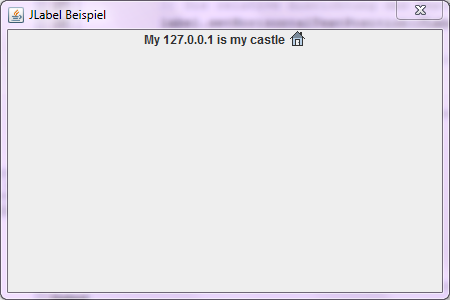
\includegraphics[scale=0.8]{images/jlabel.PNG}
		\caption{JLabel \\ \tiny{\textcolor{gray}{\url{http://http://java-tutorial.org/}}}}
		\end{figure}
\end{frame}


\subsection{JButton}
\begin{frame} %%Eine Folie
  \frametitle{JButton} %%Folientitel
  \begin{block}{Schaltfläche (Button)}
	  \begin{itemize}
		\item .
	  \end{itemize}
  \end{block}
\end{frame}

\subsubsection{Demo}
\begin{frame}
  \frametitle{Demo}
	\begin{figure}
		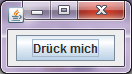
\includegraphics[scale=1.0]{images/jbutton.PNG}
		\caption{JButton \\ \tiny{\textcolor{gray}{\url{http://http://java-tutorial.org/}}}}
		\end{figure}
\end{frame}


\subsection{JToggleButton}
\begin{frame} %%Eine Folie
  \frametitle{JToggleButton} %%Folientitel
  \begin{block}{Schaltfläche, welche zwei Zustände kennt.}
	  \begin{itemize}
		\item gedrückt und nicht gedrückt
	  \end{itemize}
  \end{block}
\end{frame}


\subsubsection{Demo}
\begin{frame}
  \frametitle{Demo}
	\begin{figure}
		
\includegraphics[scale=1.0]{images/jtogglebutton_selected.PNG}
		\caption{JToggleButton Selektiert\\ \tiny{\textcolor{gray}{\url{http://http://java-tutorial.org/}}}}
		\end{figure}
\begin{figure}
		
\includegraphics[scale=1.0]{images/jtogglebutton_notselected.PNG}
		\caption{JToggleButton Nicht Selektiert \\ \tiny{\textcolor{gray}{\url{http://http://java-tutorial.org/}}}}
		\end{figure}
\end{frame}


\subsection{JCheckBox}
\begin{frame} %%Eine Folie
  \frametitle{JCheckBox} %%Folientitel
  \begin{block}{Auswahlkästchen, das, wenn es ausgewählt wurde, mit einem Häkchen oder Kreuz versehen wird.}
	  \begin{itemize}
		\item .
	  \end{itemize}
  \end{block}
\end{frame}


\subsubsection{Demo}
\begin{frame}
  \frametitle{Demo}
	\begin{figure}
		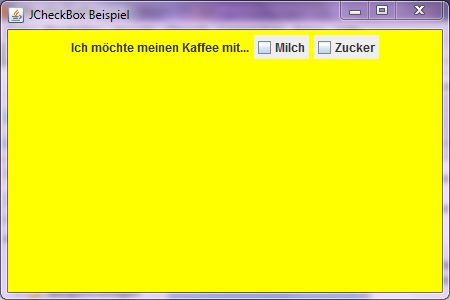
\includegraphics[scale=0.8]{images/jcheckbox.PNG}
		\caption{JCheckBox \\ \tiny{\textcolor{gray}{\url{http://http://java-tutorial.org/}}}}
		\end{figure}
\end{frame}


\subsection{JRadioButton}
\begin{frame} %%Eine Folie
  \frametitle{JRadioButton} %%Folientitel
  \begin{block}{Schaltfläche zur Auswahl zwischen mehreren Optionen, in der Regel sind sie in einer ButtonGroup angeordnet. Im Gegensatz zur JCheckBox kann nur maximal eine Option selektiert werden.}
	  \begin{itemize}
		\item .
	  \end{itemize}
  \end{block}
\end{frame}

\subsubsection{Demo}
\begin{frame}
  \frametitle{Demo}
	\begin{figure}
		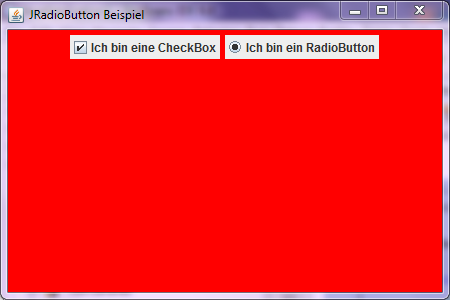
\includegraphics[scale=0.8]{images/jradiobutton.PNG}
		\caption{JRadioButton \\ \tiny{\textcolor{gray}{\url{http://http://java-tutorial.org/}}}}
		\end{figure}
\end{frame}


\subsection{JComboBox}
\begin{frame} %%Eine Folie
  \frametitle{JComboBox} %%Folientitel
  \begin{block}{Dropdown-Liste (auch als Auswahlliste oder Listbox bezeichnet), die zur Auswahl eines Elementes aufgeklappt wird. Wenn die JComboBox editierbar ist, kann über ein Textfeld der ausgewählte Wert auch vom Anwender gesetzt werden.}
	  \begin{itemize}
		\item .
	  \end{itemize}
  \end{block}
\end{frame}

\subsubsection{Demo}
\begin{frame}
  \frametitle{Demo}
	\begin{figure}
		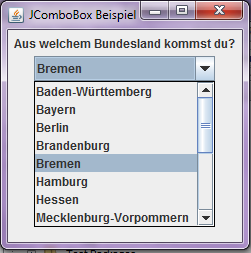
\includegraphics[scale=0.8]{images/jcombobox.PNG}
		\caption{JComboBox \\ \tiny{\textcolor{gray}{\url{http://http://java-tutorial.org/}}}}
		\end{figure}
\end{frame}


\subsection{JList}
\begin{frame} %%Eine Folie
  \frametitle{JList} %%Folientitel
  \begin{block}{Einfache Liste, die mehrere Elemente enthalten kann. Einfach- und Mehrfachauswahl möglich.}
	  \begin{itemize}
		\item .
	  \end{itemize}
  \end{block}
\end{frame}

\subsubsection{Demo}
\begin{frame}
  \frametitle{Demo}
	\begin{figure}
		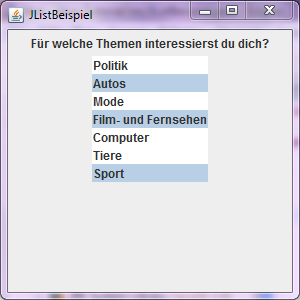
\includegraphics[scale=0.8]{images/jlist.PNG}
		\caption{JList \\ \tiny{\textcolor{gray}{\url{http://http://java-tutorial.org/}}}}
		\end{figure}
\end{frame}



\subsection{JTextField}
\begin{frame} %%Eine Folie
  \frametitle{JTextField
} %%Folientitel
  \begin{block}{einfache einzeilige Texteingabe}
	  \begin{itemize}
		\item .
	  \end{itemize}
  \end{block}
\end{frame}


\subsubsection{Demo}
\begin{frame}
  \frametitle{Demo}
	\begin{figure}
		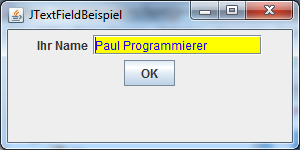
\includegraphics[scale=0.8]{images/jtextfield.PNG}
		\caption{JTextField \\ \tiny{\textcolor{gray}{\url{http://http://java-tutorial.org/}}}}
		\end{figure}
\end{frame}

\subsection{JTextArea}
\begin{frame} %%Eine Folie
  \frametitle{JTextArea
} %%Folientitel
  \begin{block}{einfache mehrzeilige Texteingabe}
	  \begin{itemize}
		\item .
	  \end{itemize}
  \end{block}
\end{frame}

\subsubsection{Demo}
\begin{frame}
  \frametitle{Demo}
	\begin{figure}
		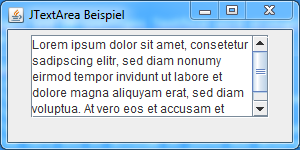
\includegraphics[scale=1.0]{images/jtextarea.PNG}
		\caption{JTextArea \\ \tiny{\textcolor{gray}{\url{http://http://java-tutorial.org/}}}}
		\end{figure}
\end{frame}


\subsection{JScrollBar}
\begin{frame} %%Eine Folie
  \frametitle{JScrollBar
} %%Folientitel
  \begin{block}{Schieberregler zum Scrollen.}
	  \begin{itemize}
		\item .
	  \end{itemize}
  \end{block}
\end{frame}


\subsubsection{Demo}
\begin{frame}
  \frametitle{Demo}
	\begin{figure}
		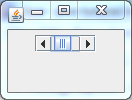
\includegraphics[scale=1.0]{images/jscrollbar.PNG}
		\caption{JScrollBar \\ \tiny{\textcolor{gray}{\url{http://http://java-tutorial.org/}}}}
		\end{figure}
\end{frame}


\subsection{JSlider}
\begin{frame} %%Eine Folie
  \frametitle{JSlider
} %%Folientitel
  \begin{block}{Schieberregler, der mit einer Skala versehen werden kann.}
	  \begin{itemize}
		\item .
	  \end{itemize}
  \end{block}
\end{frame}

\subsubsection{Demo}
\begin{frame}
  \frametitle{Demo}
	\begin{figure}
		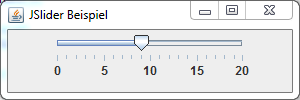
\includegraphics[scale=1.0]{images/jslider.PNG}
		\caption{JSlider \\ \tiny{\textcolor{gray}{\url{http://http://java-tutorial.org/}}}}
		\end{figure}
\end{frame}


\subsection{JProgressBar}
\begin{frame} %%Eine Folie
  \frametitle{JProgressBar} %%Folientitel
  \begin{block}{Fortschrittsbalken}
	  \begin{itemize}
		\item .
	  \end{itemize}
  \end{block}
\end{frame}

\subsubsection{Demo}
\begin{frame}
  \frametitle{Demo}
	\begin{figure}
		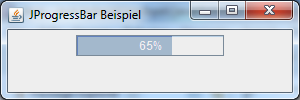
\includegraphics[scale=1.0]{images/jprogressbar.PNG}
		\caption{JProgressBar \\ \tiny{\textcolor{gray}{\url{http://http://java-tutorial.org/}}}}
		\end{figure}
\end{frame}

\subsection{JSpinner}
\begin{frame} %%Eine Folie
  \frametitle{JSpinner
} %%Folientitel
  \begin{block}{Ähnlich der JComboBox, allerdings klappt die Liste nicht auf, sondern die Navigation durch die Liste erfolgt über Pfeiltasten.}
	  \begin{itemize}
		\item .
	  \end{itemize}
  \end{block}
\end{frame}

\subsubsection{Demo}
\begin{frame}
  \frametitle{Demo}
	\begin{figure}
		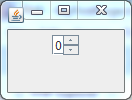
\includegraphics[scale=1.0]{images/jspinner.PNG}
		\caption{JSpinner \\ \tiny{\textcolor{gray}{\url{http://http://java-tutorial.org/}}}}
		\end{figure}
\end{frame}

\subsection{JSeparator}
\begin{frame} %%Eine Folie
  \frametitle{JSeparator
} %%Folientitel
  \begin{block}{einfache Trennlinie}
	  \begin{itemize}
		\item .
	  \end{itemize}
  \end{block}
\end{frame}

\subsubsection{Demo}
\begin{frame}
  \frametitle{Demo}
	\begin{figure}
		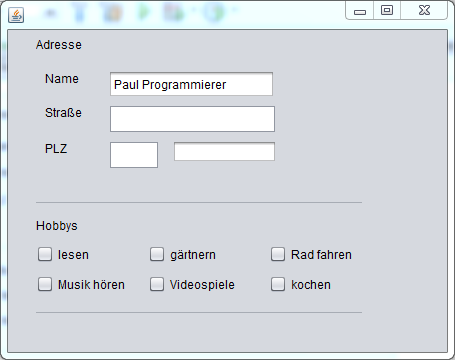
\includegraphics[scale=0.6]{images/jseparator.PNG}
		\caption{JSeparator \\ \tiny{\textcolor{gray}{\url{http://http://java-tutorial.org/}}}}
		\end{figure}
\end{frame}

\section{Anhang}
\begin{frame}
  \frametitle{Anhang} %%Folientitel
	\begin{block}{}	
		\begin{center}
			Vielen Dank für Ihre Aufmerksamkeit. \\
			Fragen?
		\end{center}	
	\end{block}
	\begin{block}{Link zum Präsentation}	
		\begin{itemize}
			\item \url{https://github.com/derdanu/akad-jav02-beamer}
		\end{itemize}
	\end{block}
\end{frame}

\subsection{Quellen}
\begin{frame} %%Eine Folie
  \frametitle{Quellen} %%Folientitel
 	\begin{itemize}
		\item \url{http://docs.oracle.com/javase/7/docs/}	
		\item \url{http://java-tutorial.org/bedienelemente.html}
	\end{itemize}
\end{frame}




\end{document}


